%% rpg-module.tex
%
% Documentation and worked example for the Role-Playing Game Module class
%
% Copyright 2017 Michael C. Davis
%
% LICENSE FOR THE WORK
%
% This work consists of the following files:
%    rpg-module.cls
%    rpg-basic-stats.sty
%    rpg-basic-stats.def
%    rpg-1e-stats.sty
%    rpg-1e-stats.def
%    doc/rpg-module.tex
%
% This work may be distributed and/or modified under the conditions of the LaTeX
% Project Public License, either version 1.3 of this license or (at your option)
% any later version. The latest version of this license can be found at:
% http://www.latex-project.org/lppl.txt
% and version 1.3 or later is part of all distributions of LaTeX version
% 2005/12/01 or later.
%
% This work has the LPPL maintenance status `author-maintained'.
% 
% The Author and Maintainer of this work is Michael C. Davis
%
%
% OPEN GAME LICENSE
%
% The monster stats in this file are copyright 2000, Wizards of the Coast, Inc.
% and are distributed with permission under the terms of the Open Game License v 1.0.
% See the file rpg-module.cls or the compiled documentation file rpg-module.pdf for
% the full text of the license.
%
%
% LICENSE FOR COMPILED WORKS
%
% You may distribute compiled works generated using the work as specified in
% Clause 3 of the LaTeX Project Public License. If you incorporate Open Gaming
% Content into the compiled work, you must also comply with the terms of that
% license.
%
%
% USAGE
%
% In addition to this documentation, there are a number of worked examples in the
% examples/ directory.
%
% Technical support is provided on GitHub:
%
%    https://github.com/slithy/rpg_module
%
% and on the Dragonsfoot Forums:
%
%    http://www.dragonsfoot.org/forums/viewtopic.php?f=87&t=73823

%% Start here!
%
% Load the rpg-module class. The following options are available:
%
% a4paper         Use A4 paper size (default)
% letterpaper     Use US letter paper size
% sansserif       Use URW Gothic font (similar to ITC Avant Garde Gothic) (default)
% serif           Use ITC Souvenir if available, fall back to URW Bookman if not available
% acdesc          Use descending AC in stat blocks
% acasc           Use ascending AC in stat blocks
% acb1            Use B1-style AC in stat blocks (inspired by http://zenopusarchives.blogspot.com/2014/02/ascending-ac-in-holmes-basic.html)
% acsw            Use Swords & Wizardry style AC in stat blocks
% basic           Use Basic stat blocks (default)
% 1e              Use Advanced stat blocks (not currently implemented, planned for a future release)
%
% In principle, stat blocks can be defined for any RPG system by defining the appropriate style file.
% In this release of the class, only rpg-basic-stats.sty is defined.

%\documentclass[a4paper,serif]{rpg-module}
\documentclass[a4paper,sansserif]{rpg-module}

\usepackage{lipsum}                                                             % This package generates filler text for
                                                                                % the example file, not needed in a real project

%\usepackage{parskip}                                                           % add spacing between paras instead of indents



\begin{document}

%% TITLE PAGE %%
%
% If you want a title page, define the elements you want, then use \maketitle (see below).
%
% It is required to define \title, even without a title page, as it is used for running heads for A4 paper size.

\title{Dungeon Module X2$\varepsilon$\\
An Adventure Module Class and Template}

% The rest of the title page elements are optional

\author{Michael C. Davis}

\titlerunning{Dungeon Module X2$\varepsilon$ : Module Class}                     % Shorter title for running heads (A4 paper option only)

\subtitle{Introductory module for character levels 1--3}

\coverimage{rpg-module-cover-art.png}

\abstract{This template is inspired by the old-school modules of the 1980s. It is an attempt to recapture the look and feel
of those classic adventures using the power and beauty of the \LaTeX~typesetting system. The template is designed to allow
authors to typeset their adventures with a minimum of effort. Write your adventure, add some simple markup notation as shown
in the example file, and in a few clicks you will have a beautifully-formatted PDF.}

\copyrightblock{The \LaTeX~rpg-module class is Copyright \copyright 2016 Michael Davis and is distributed under the terms
of the \href{http://www.latex-project.org/lppl.txt}{LaTeX Project Public License} (LPPL) Version 1.3c. You are free to use this
class to generate works for distribution, for free or commercially, as detailed in Clause 3 of the license.

Some parts of the template are Copyright \copyright 2000--2003 Wizards of the Coast and are distributed under the
\hyperref[ogl]{Open Game License (OGL)} Version 1.0A.

The images and maps in this example template are not covered by the LPPL. See the license for each work.}

% The contact block is to typeset your logo(s), company name and/or contact details. It consists of three columns; you
% can use any or all of them. By default the columns are top-aligned and of equal width, but you can redefine this in the
% optional argument. See the documentation of the LaTeX tabular environment for details.

\contactblock[p{2.9cm} p{5.0cm} p{9.8cm}]{% column 1 : logo
\begin{center}

\includegraphics[width=1.5cm]{rpg-module-logo.png}
\end{center}
}{% column 2 : empty in this example
}{% column 3 : contact details
\vspace{0.4cm}
\begin{flushright}
The author can be contacted on Dragonsfoot (user:
\href{http://www.dragonsfoot.org/forums/ucp.php?i=pm&mode=compose&u=7317}{slithy}).\\[0.5em]

Support for the rpg-module class and this template is provided on
\href{https://github.com/slithy/rpg_module}{GitHub} and the
\href{http://www.dragonsfoot.org/forums/viewtopic.php?f=87&t=73823}{Dragonsfoot Computer Gaming \& Utilities} forum.
\end{flushright}
}

% Typeset the title page from the elements above. Remove \maketitle if you don't want a title page.

\maketitle



%% START OF PAGE 1 %%
%
% Display the title text again at the top of the first column.
% Or, use \showtitle[newtext] to use newtext in place of the previously-defined title.

\showtitle

This file is a tutorial and example of how to use the rpg-module class to typeset your fantasy role-playing game adventure.

\part{Introduction}

The rpg-module class is a free resource for authors of adventure modules for fantasy roleplaying games.
It is inspired by the look and feel of the 1981 ``Red Book'' Basic incarnation of the world's most popular FRPG.

To prepare your work using this class, you will need \LaTeX, a free document preparation system for high-quality
typesetting. The rpg-module class was developed and tested using \TeX Live, which you can download from
\href{https://latex-project.org/ftp.html}{the \LaTeX~Project website}.

Unlike a conventional word processor, the \LaTeX~philosophy is to separate the job of writing and editing content
from the job of typesetting it for publication. Authors can concentrate on writing their text without fussing
about what fonts to choose or what size the page margins or table columns should be. The rpg-module class takes care
of all that. Another advantage is that all documents produced using this template will have a similar look and
feel, so if you want to publish a series of works they will appear consistent.

\LaTeX~uses a markup language in order to describe document structure and presentation. This
file---\verb|rpg-module.pdf|---was created from the markup file \verb|rpg-module.tex|. If you open \verb|rpg-module.tex|
in an ordinary text editor, you will see the markup commands and some explanatory comments (prefixed by \%).
\LaTeX~converts your source text, combined with the markup and the rpg-module class, into a high quality PDF document.

You can find numerous tutorials online to get you started with the basics of document preparation using \LaTeX.
Part~\ref{using_the_module_class} of this document explains the features of the rpg-module class. Part~\ref{example_dungeon}
is an example of how to create a dungeon module using the class.

\part{Using the Module Class}
\label{using_the_module_class}

\section{Class Options}

At the beginning of your document, load the rpg-module class with \verb|\documentclass[<options>]{rpg-module}|. You can
specify the following options:

\begin{tabularx}{\linewidth}{lX}
\verb|a4paper|      & Use A4 paper size (default)\\
\verb|letterpaper|  & Use US letter paper size\\
\verb|sansserif|    & Use a sans-serif font, URW Gothic (default).\\
\verb|serif|        & Use a serifed font. This option will use ITC Souvenir if available, URW Bookman otherwise.\\
\verb|tightsqueeze| & Reduce the spacing between table rows and around headings for a more compact layout.\\
\verb|acdesc|       & Use descending AC in stat blocks (default for Basic stats)\\
\verb|acasc|        & Use ascending AC in stat blocks\\
\verb|acb1|         & Use \href{http://zenopusarchives.blogspot.com/2014/02/ascending-ac-in-holmes-basic.html}{the B1 AC style} in stat blocks\\
\verb|acsw|         & Use \href{http://www.swordsandwizardry.com/}{Swords \& Wizardry} AC style in stat blocks\\
\verb|basic|        & Use Basic monster stat blocks (default)\\
\verb|1e|           & Use Advanced 1st Edition monster stat blocks\\
\end{tabularx}

\subsection*{Paper Size}

rpg-module supports the letter paper size (used in USA) and A4 (used in Europe and the rest of the world). Changing the paper size
does not scale the text on the page; rather it adjusts the margins so the pages will be typeset identically regardless
of which size is selected. This allows module writers to easily create two almost identical PDFs for use in different regions.

As A4 pages are slightly taller, you have the option of a running header if you select \verb|a4paper|. This option is not available
in Letter paper size.

\subsection*{Fonts}

You can select a serifed or sans-serif font. The default font is URW Gothic (sans-serif), a free font which is similar to
ITC Avant Garde Gothic. Avant Garde was used in many early TSR modules, including B1 and B2.

If you choose the serif option, the rpg-module class will try to use ITC Souvenir. Souvenir is used for the 1981 Basic rulebook
and modules including B3 (Green cover), X1 and X2. However, it is a commercial font which is
not distributed with \LaTeX. If you don't have Souvenir installed, the rpg-module class will use URW Bookman instead, which is
included in the standard \TeX Live distribution.

If you want to obtain the Souvenir font, note that it was bundled with some versions of CorelDraw. It is more economical to buy
CorelDraw with its bundled font license than to buy the font directly from the foundry.
To configure the font for use with \LaTeX, you need the Adobe Type 1 font definitions (.pfb and .afm files) from CorelDraw
and the corresponding LaTeX .tfm and .vf files, which you can obtain from the \href{https://www.ctan.org/pkg/corelpak}{Corelpak} package. The
\href{https://www.ctan.org/pkg/corelpak-contrib}{Corelpak-contrib} package may also be useful to help with installation.

\subsection*{Stat Blocks}

The rpg-module class is designed to be extensible. This version of the class includes Basic-style monster stat blocks
(\verb|basic|) and Advanced 1st Edition-style monster stat blocks (\verb|1e|). See p.\pageref{stat_blocks} for more detail.

In principle it is possible to define a new stat block format for any RPG system. If several systems are defined, authors
can compile the same work with stats for different systems simply by changing the option passed to \verb|documentclass|.

\section{Layout Options}

\subsection*{Headings}

The defined heading styles are listed in Table~\ref{tab:heading_styles}.
If you want a table of contents in your document, simply place a \verb|\tableofcontents| command where you would like it to appear.

\begin{table}[ht]
\begin{tabularx}{\linewidth}{lp{0.25\linewidth}>{\raggedright\arraybackslash}X}
\tableheader{Style                     & Description                 & Features}
\texttt{\textbackslash part}           & Chapter heading             & Numbered, included in table of contents (ToC)\\
\texttt{\textbackslash section}        & Section heading             & Not numbered, left justified, upper case, included in ToC\\
\texttt{\textbackslash section*}       & Section heading (alternate) & Not numbered, centred, included in ToC\\
\texttt{\textbackslash subsection}     & Location key                & Numbered, not included in ToC\\
\texttt{\textbackslash subsection*}    & Subheading/Table heading    & Not numbered, not included in ToC\\
\texttt{\textbackslash subsubsection}  & Sub-location key            & Numbered with number and letter: ``7a.'' Not included in ToC\\
\texttt{\textbackslash subsubsection*} & Sub-location key            & Not numbered, not included in ToC\\
\end{tabularx}
\caption{Heading Styles}
\label{tab:heading_styles}
\end{table}

Location keys are numbered automatically starting from 1, and numbering is restarted after each section heading. You can override
the default numbering using the \verb|\setcounter| macro. For example, to continue the location key numbering starting at 20 on the
second level of your dungeon, insert \verb|\setcounter{subsection}{19}| before the first subsection heading on level 2.

\subsection*{Boxed Text}

To draw a box around any text, enclose it in the \verb|boxtext| environment:

\begin{boxtext}
Lorem ipsum dolor sit amet, consectetuer adipiscing elit. Ut
purus elit, vestibulum ut, placerat ac, adipiscing vitae, felis.
Curabitur dictum gravida mauris. Nam arcu libero, nonummy
\end{boxtext}

\subsection*{Tables}

The rpg-module class uses the standard \verb|tabular| environment for tables. It defines a new \verb|\tableheader| macro which centres
the table headings and writes a horizontal rule of the correct width under each one, in the same style as the Basic rulebook.

You need to specify the number and format of each column in your table as usual: \verb|l| for left-aligned, \verb|c| for centred
and \verb|r| for right-aligned. The class also provides a new \verb|b| column type for bold, centred headings.

Here is an example. The table below has two columns: one centred and one left-aligned. So the table format
is defined using \verb|\begin{tabular}{cl}|. The heading rows are defined as bold and centred: \verb|\tableheader[b]{Damage & Weapon Type}|.

\section*{New Weapon Damage Table}

\begin{center}
\begin{tabular}{cl}
\tableheader[b]{Damage & Weapon Type}
1-4 (1d4) & Throwing Stick\\
1-6 (1d6) & Composite Bow\\
1-4 (1d4) & Cutting Axe\\
1-6 (1d6) & Piercing Axe\\
1-8 (1d8) & Khopesh\\
6-36 (6d6) & Chariot\\
\end{tabular}
\end{center}

If you need to squeeze wide tables into a text column, you can control the inter-column spacing using \verb|\tabcolsep|,
like this:

\section*{Character Attacks}

\begin{center}
\addtolength{\tabcolsep}{-4.1pt}
\begin{tabular}{lccccccccccccc}
\tableheader{Attacker's Level & 9 & 8 & 7 & 6 & 5 & 4 & 3 & 2 & 1 & 0 & -1 & -2 & -3}
Normal man & 11 & 12 & 13 & 14 & 15 & 16 & 17 & 18 & 19 & 20 & 20 & 20 & 20\\
1st to 3rd & 10 & 11 & 12 & 13 & 14 & 15 & 16 & 17 & 18 & 19 & 20 & 20 & 20\\
4th + higher & 8 & 9 & 10 & 11 & 12 & 13 & 14 & 15 & 16 & 17 & 18 & 19 & 20\\
\end{tabular}
\addtolength{\tabcolsep}{4.1pt}
\end{center}

\vspace{1ex}\noindent The rpg-module class also defines two special-purpose tables: the Wandering Monster table and Monster Roster table. These tables
have pre-defined headings and each line is populated using a monster stat block (see the next section).

\noindent Wandering Monster tables are defined with:
\begin{quote}
\verb|\begin| \verb|{wanderingmonsters}[style]|
\end{quote}
The optional \verb|[style]| argument specifies the column type for headers. The \verb|[b]| style uses the same bold,
centred style used for the New Weapon Damage Table above. Each line of the Wandering Monster table is defined using:
\begin{quote}
\verb|\wanderitem[die roll]{monstername}{no. appearing}|
\end{quote}
\verb|[die roll]| is optional; if you omit it, each row will be numbered consecutively starting at 1. If you want to
roll 2d6 for wandering monster determination, then put \verb|[2]| on the first row and the following rows will be numbered
consecutively. Or if you want to use ranges, you can specify the range for each line like this: \verb|[01--10]|.
(A point of typographic pedantry: in \LaTeX, two hyphens will be typeset as an en-dash, ``--'', which is the correct length
of dash to use for numeric ranges. For parenthetical dashes use three hyphens to get the longer em-dash, ``---'').

\verb|{monstername}| is the key for the stat block; see the next section for an explanation.
\verb|{no. appearing}| is optional; if you leave it empty, the rpg-module class will use the default number appearing as defined in the stat block.

The Monster Roster table is similar, but the table headings are slightly different. Define the table with:
\begin{quote}
\verb|\begin{monsterroster}[style]|
\end{quote}
The first column is the location key, and there is an extra column for hit points. Each line in
the table is defined using:
\begin{quote}
\hspace{-2em}\verb|\rosteritem{locationkey}{monstername}{number}{hitpoints}|
\end{quote}
If the location key is defined as a \LaTeX~reference, the class will generate the correct location number and create a hyperlink to that section.

You can see examples of Wandering Monster and Monster Roster tables on p.\pageref{wanderingmonsters}.

\section{Monster Stat Blocks}
\label{stat_blocks}

The Basic stats style included with the rpg-module class has stats for all of the monsters in the Basic and Expert rulebooks.
To typeset a statblock, simply use:
\begin{quote}
\verb|\statblock{monstername}{noappearing}{hitpoints}|
\end{quote}
The rpg-module class will work out the correct singular or plural forms automatically, so
\verb|\statblock{gnoll}{1}{10}| gives:
\statblock{gnoll}{1}{10}
while \verb|\statblock{gnoll}{5}{16,14,12,9,8}| gives:
\statblock{gnoll}{5}{16,14,12,9,8}
If you prefer, there is also an inline style:
\begin{quote}
\hspace{-2em}\verb|\stats[description]{monstername}{noappearing}{hitpoints}|
\end{quote}
where the optional \verb|[description]| overrides the default name of the monster.
For example:\\[0.1em]

\noindent You find yourself face to face with the \stats[Gnoll Chieftain!]{gnoll}{1}{16}. He is flanked
by \stats[12 bodyguards: ]{gnoll}{12}{10 each}.\\[0.1em]

\noindent You can of course also define new monsters beyond those in the Basic and Expert rulebooks. Define the new
monster once at the beginning of your document, and then you can use it in the same way as the predefined
monsters above. The format for a new monster definition is:
\begin{quote}
\verb|\monster[pluralname]{label}{name}{stats}|
\end{quote}
where \verb|label| is the key you want to use for the monster (\verb|gnoll| in the examples above) and
\verb|name| is the (singular) name of the monster that will be displayed in the text, ``Gnoll''. The rpg-module
class can usually work out the plural form by following some simple rules, but if the plural is unusual,
you can specify it in the optional \verb|pluralname| field. For example, if you define:
\begin{quote}
\verb|\monster{octopus}{Octopus}{|\ldots
\end{quote}
you will get the default plural, ``Octopuses''. If you decide that the plural should instead be ``Octopodes'', you can override the default definition:
\begin{quote}
\verb|\monster[Octopodes]{octopus}{Octopus}{|\ldots
\end{quote}

\noindent The \verb|stats| field is a list of the monster stats, separated by ``\verb:|:''. It should contain the following items in order:
\renewcommand{\labelitemi}{$\bullet$}
\begin{itemize}\setlength{\itemsep}{0pt}
\item Type. This is only required where the monster is a subspecies of a general type, e.g. ``Dragon'', ``Lycanthrope'' or ``Man''. In all other cases
it should be left blank.
\item Put an asterisk (*) in this column if the monster requires silver, magic or special weapons to hit it. Leave empty otherwise.
\item \ArmourClass. This should be in descending AC format; use the \verb|acasc| option to the class if you want to convert it to ascending AC.
\item Hit Dice (including * or ** if applicable)
\item Movement per Turn
\item Movement per Round
\item Special Movement class, e.g. ``Fly'' or ``Swim''. Leave blank in most cases.
\item Special Movement per Turn
\item Special Movement per Round
\item Attacks (short form). Usually just the number of attacks, or ``3+special''. This format is used only in Wandering Monster and Monster Roster tables.
\item Attacks (long form). More verbose description of attacks, used in New Monster listing and stat blocks, e.g. ``2 claws\?bite\+breath''.
\footnote{Note that the slash character \texttt{/} is non-breaking (\LaTeX~will not place a line break after \texttt{/}). The rpg-module class provides a breaking
slash \texttt{\textbackslash ?} to overcome this problem. The class also provides \texttt{\textbackslash +}, which is a breaking version of +. Use of
\texttt{\textbackslash ?} and \texttt{\textbackslash +} in the long attack and damage fields prevents awkward line breaks in stat blocks.}
\item Damage (short form). Used in Wandering Monster and Monster Roster tables.
\item Damage (long form). Used in New Monster listing and stat blocks.
\item Save As. List the long form, e.g. ``Fighter: 3''. The short form is computed where required.
\item Morale
\item Alignment. List the long form, e.g. ``Chaotic''. The short form is computed where required. In case of monsters with variable alignment, specify ``Any''
here, and use the \verb|\changealignment| macro to specify as needed in the text. (For example, the Acolyte is defined with alignment Any but is given a specific
alignment in the Wandering Monster table on p.\pageref{wanderingmonsters}.)

\item No. Appearing. List the range when encountered as a wandering monster.
\item No. Appearing in Lair. List the range when encountered in the monster's lair or in the wilderness.
\item Treasure Type
\item XP
\end{itemize}

\noindent For example, suppose we create the following definition:\\[0.1em]

\begin{ifbasicstats}
\monster[Minions of Set]{minion_set}{Minion of Set}{||0|5**|120'|40'||||1/1|weapon or bite or by form|1d8/1d12+poison|1d8 or 1d12+poison or by form|Fighter: 10|12|Chaotic|1--6|1--20|Nil|425}
\end{ifbasicstats}
\begin{if1estats}
% \monster{key}[Name, Plural]{Name, Singular}{Type|THAC0|AC|MV|HD|Attacks|Dmglong|Dmg|SA|SD|MR|Special|SZ|Int|AL|Psi|PsiAtt|Frequency|NoAppear|InLair|TT|Level|XP}
\monster[Minions of Set]{minion_set}{Minion of Set}{|12|\minus 2|12"|F10|3/2|1--12 (bite), by weapon type, or by form|1--12|Polymorph, poison bite|Save as 10th level Fighter|10\%|Polymorph, poison bite|M|High|Lawful Evil|Nil|Nil|Uncommon|1--20|0\%|Nil|V|500}
\end{if1estats}

\noindent\texttt{\textbackslash monster[Minions~of~Set]\{minion\_set\}\{Minion~of~Set\}\{||0|
5**|120'|40'||||1/1|weapon~or~bite~or~by~form|
1d8/1d12+poison|1d8~or~1d12+poison~or~by~form|
Fighter:~10|12|Chaotic|1--6|1--20|Nil|425\}}\\[0.1em]

\noindent Now any time we want to put stats for a Minion of Set in our text, we can use a definition like this:
\begin{quote}
\verb|\statblock{minion_set}{4}{25 each}|
\end{quote}
which produces a stat block like this:
\statblock{minion_set}{4}{25 each}
You can add details of your new monster with the environment:
\begin{quote}
\verb|\begin{newmonster}{minion_set}|
\verb|Text description of your monster here|\ldots\\
\verb|\end{newmonster}|
\end{quote}
You can see an example of what this looks like on p.\pageref{minion_set}.

If you want to redefine an existing monster, you can do so using exactly the same commands.

Finally, there is the \verb|statblockfreestyle| environment. This should be used sparingly; for most monsters, you should use
the standard macros to ensure consistency. However, sometimes you may want to include extra information which does not
fit into the standard stat blocks, such as the attributes of NPCs or spell lists:

% Define the standard stat block as well for use in tables

\begin{ifbasicstats}
\monster{snefru_hotep}{Snefru-Hotep}{||5|C5|90'|30'||||1|mace or spell|1d6/spell|1d6 or spell|Cleric: 5|11|Chaotic|1|1|Nil|300}
\end{ifbasicstats}
\begin{if1estats}
% \monster{key}[Name, Plural]{Name, Singular}{Type|THAC0|AC|MV|HD|Attacks|Dmglong|Dmg|SA|SD|MR|Special|SZ|Int|AL|Psi|PsiAtt|Frequency|NoAppear|InLair|TT|Level|XP}
\monster{snefru_hotep}{Snefru-Hotep}{|18|5|9"|C5|1|1d6 (mace)|1d6|spell use||Nil|Spell use|M|Average|Lawful Evil|Nil|Nil|Unique|1|n/a|Special|V|300}
\end{if1estats}

\begin{statblockfreestyle}
\begin{ifbasicstats}
Snefru-hotep, Cleric of Set, S9 I15 W17 D10 C8 Ch15. AC 5 (chain mail), C5, hp 21, MV 90'\,(30'), Att mace, D 1--6, Save C5, ML 11, AL C.
He can cast the following spells: Protection from Good, Cause Fear, Snake Charm, Hold Person.
\end{ifbasicstats}
\begin{if1estats}
Snefru-hotep, Cleric of Set, S9 I15 W17 D10 C8 Ch15. AC 5 (chain mail), C5, hp 21, MV 9", Att mace, D 2--7, AL LE.
He can cast the following spells: Protection from Good, Cause Fear, Cause Light Wounds ($\times 2$), Darkness,
Snake Charm, Hold Person, Slow Poison, Spiritual Hammer, Speak with Animals, Animate Dead, Curse.
\end{if1estats}
\end{statblockfreestyle}

\noindent When using \verb|statblockfreestyle|, the rpg-module class provides \verb|ifbasicstats| and \verb|if1estats| macros to specify separate
stat blocks for different RPG systems.

The rest of this document shows a full example of how an adventure can be typeset using the rpg-module class.

\newpage

%%%%% Level One %%%%%

% Float the map on a page on its own

\begin{figure*}[p]
\centering
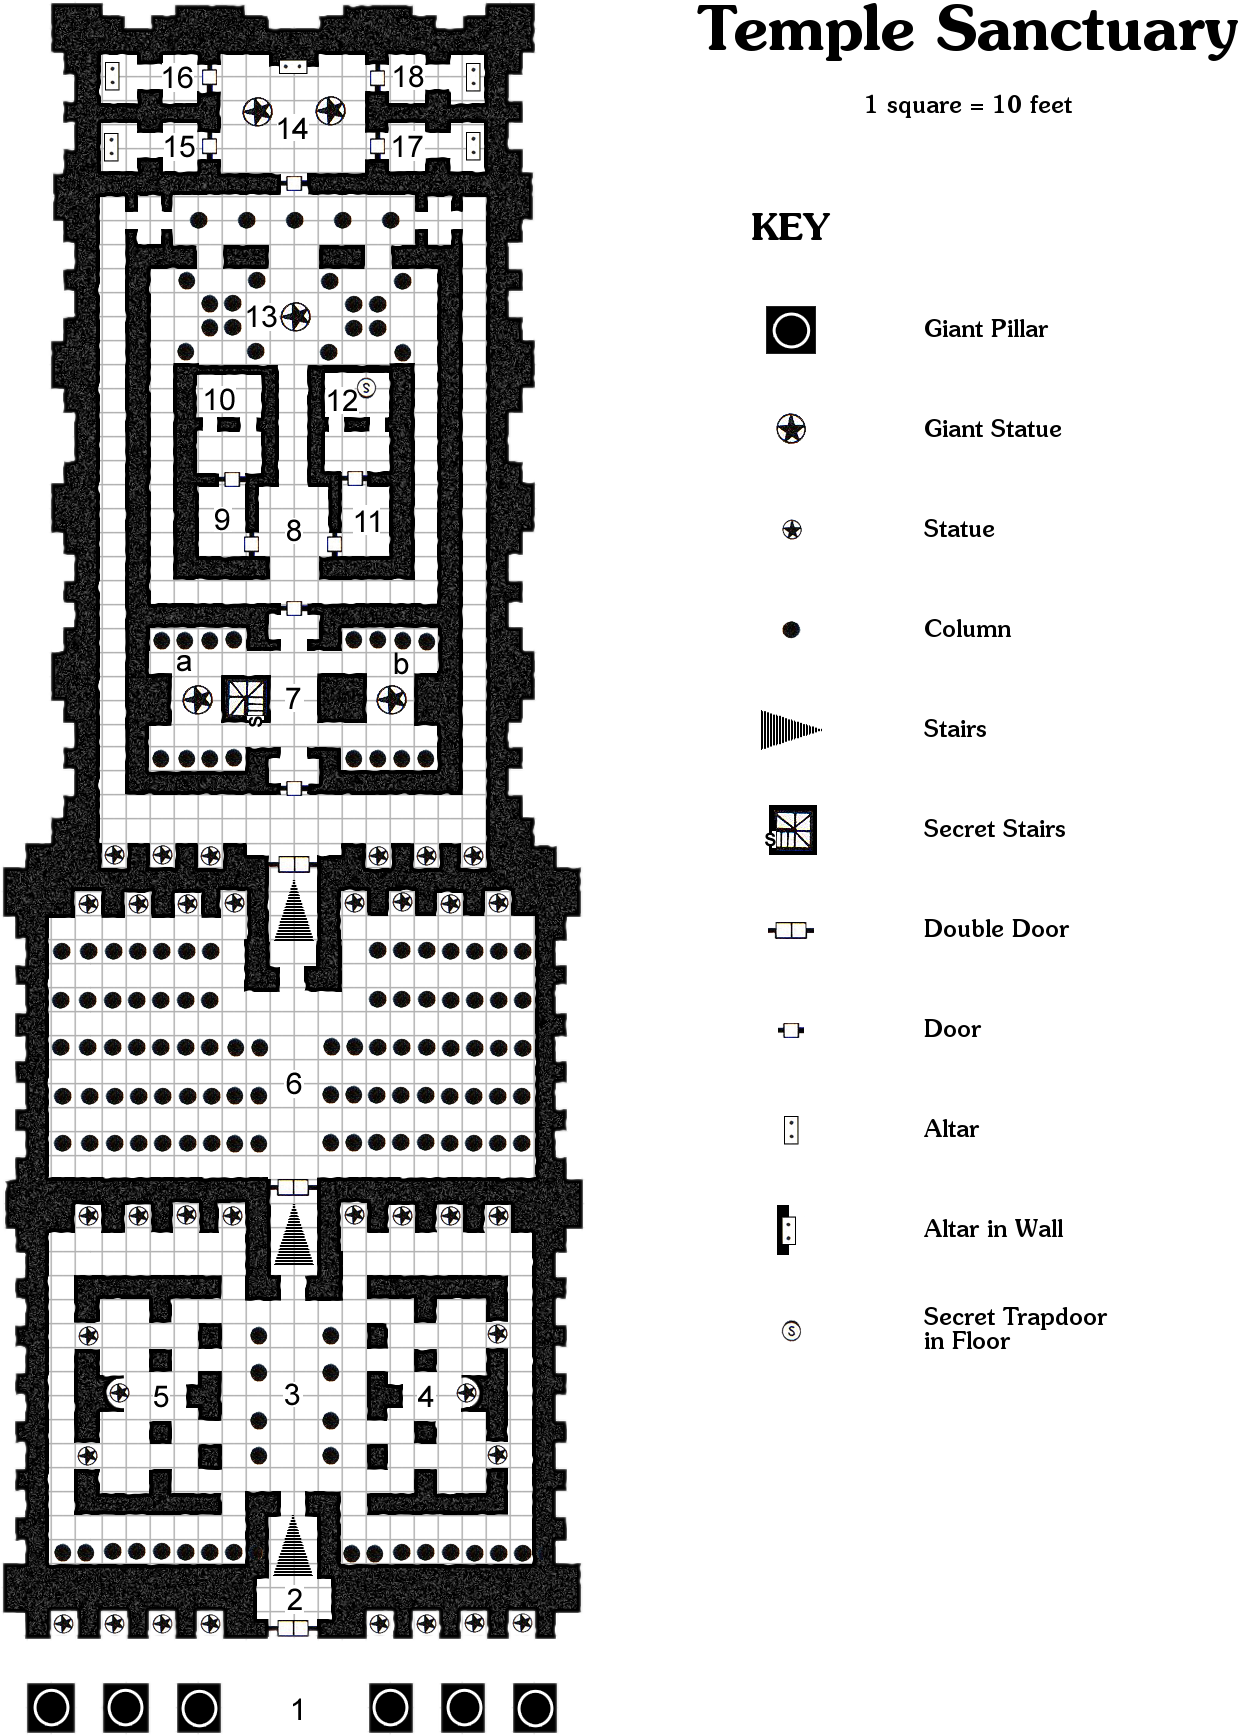
\includegraphics[width=0.75\textwidth]{rpg-module-map.png}
\vspace{5ex}
\caption*{Map Copyright \copyright 2008, 2016 Tim Hartin of
\href{http://paratime.ca}{Paratime Design}. Used with permission. All rights reserved.}
\label{img:map}
\end{figure*}

\part{First Dungeon Level}
\label{example_dungeon}

\section*{Key to Dungeon Level One}

\subsection*{Start}

\begin{boxtext}
You have traveled across the desert for many days. Ahead in the distance you can see a large stone
structure rising above the sand.
\end{boxtext}

The structure is the fabled Temple of Set. Within, the evil priests of Set plan world domination.
A tribe of gnolls revere the site and guard the outer precincts.

\subsection{The Portico} % Key 1
\label{portico}

The gnolls do not live within the temple; their settlement is a short distance away. But every day they
send a small delegation to petition the priests and seek the power of Set. They will be hostile towards
strangers.

\begin{boxtext}
The building is made of cyclopean blocks of granite rising above the desert sands. You wonder how such
an edifice could have been constructed here, so far from any obvious habitation. Surely thousands of
workers---slaves in all probability---must have been employed in building it.

The facade of the edifice is some 150' across. Huge stone steps lead up to a portico, which is flanked
by six immense pillars.
\end{boxtext}

There are 13 steps, each 3' tall and thus difficult to climb. The pillars are embossed with heiroglyphs
which (could the players read them), tell the story of Set's rise to power, his conquests and the
bitter enmity which exists between him and his brother Osiris.

On the porch at the top of the stairs, a group of Gnoll petitioners keep watch. When they perceive
the party from afar, they will hide behind the pillars. As the party begin to mount the steps, they will
spring out and hurl their javelins (1d6+1 dmg). They are also armed with spiked clubs:
\statblock{gnoll}{6}{9 each}
The gnolls each carry 1d4 ep and 2d10 cp.

On the porch, behind the pillars and not visible from below, are eight statues\ldots

\subsection{Vestibule} % Key 2

\begin{boxtext}
\lipsum[1]
\end{boxtext}

\lipsum[2]

\subsection{Central Aisle} % Key area 3

\begin{boxtext}
\lipsum[3]
\end{boxtext}

\lipsum[4]

\subsection{East Court} % Key area 4

\lipsum[5]

\subsection{West Court} % Key area 5

\lipsum[6]

\subsection{Great Hypostyle Hall} % Key area 6
\label{hypostyle_hall}

% Floating image

\begin{figure}[t]
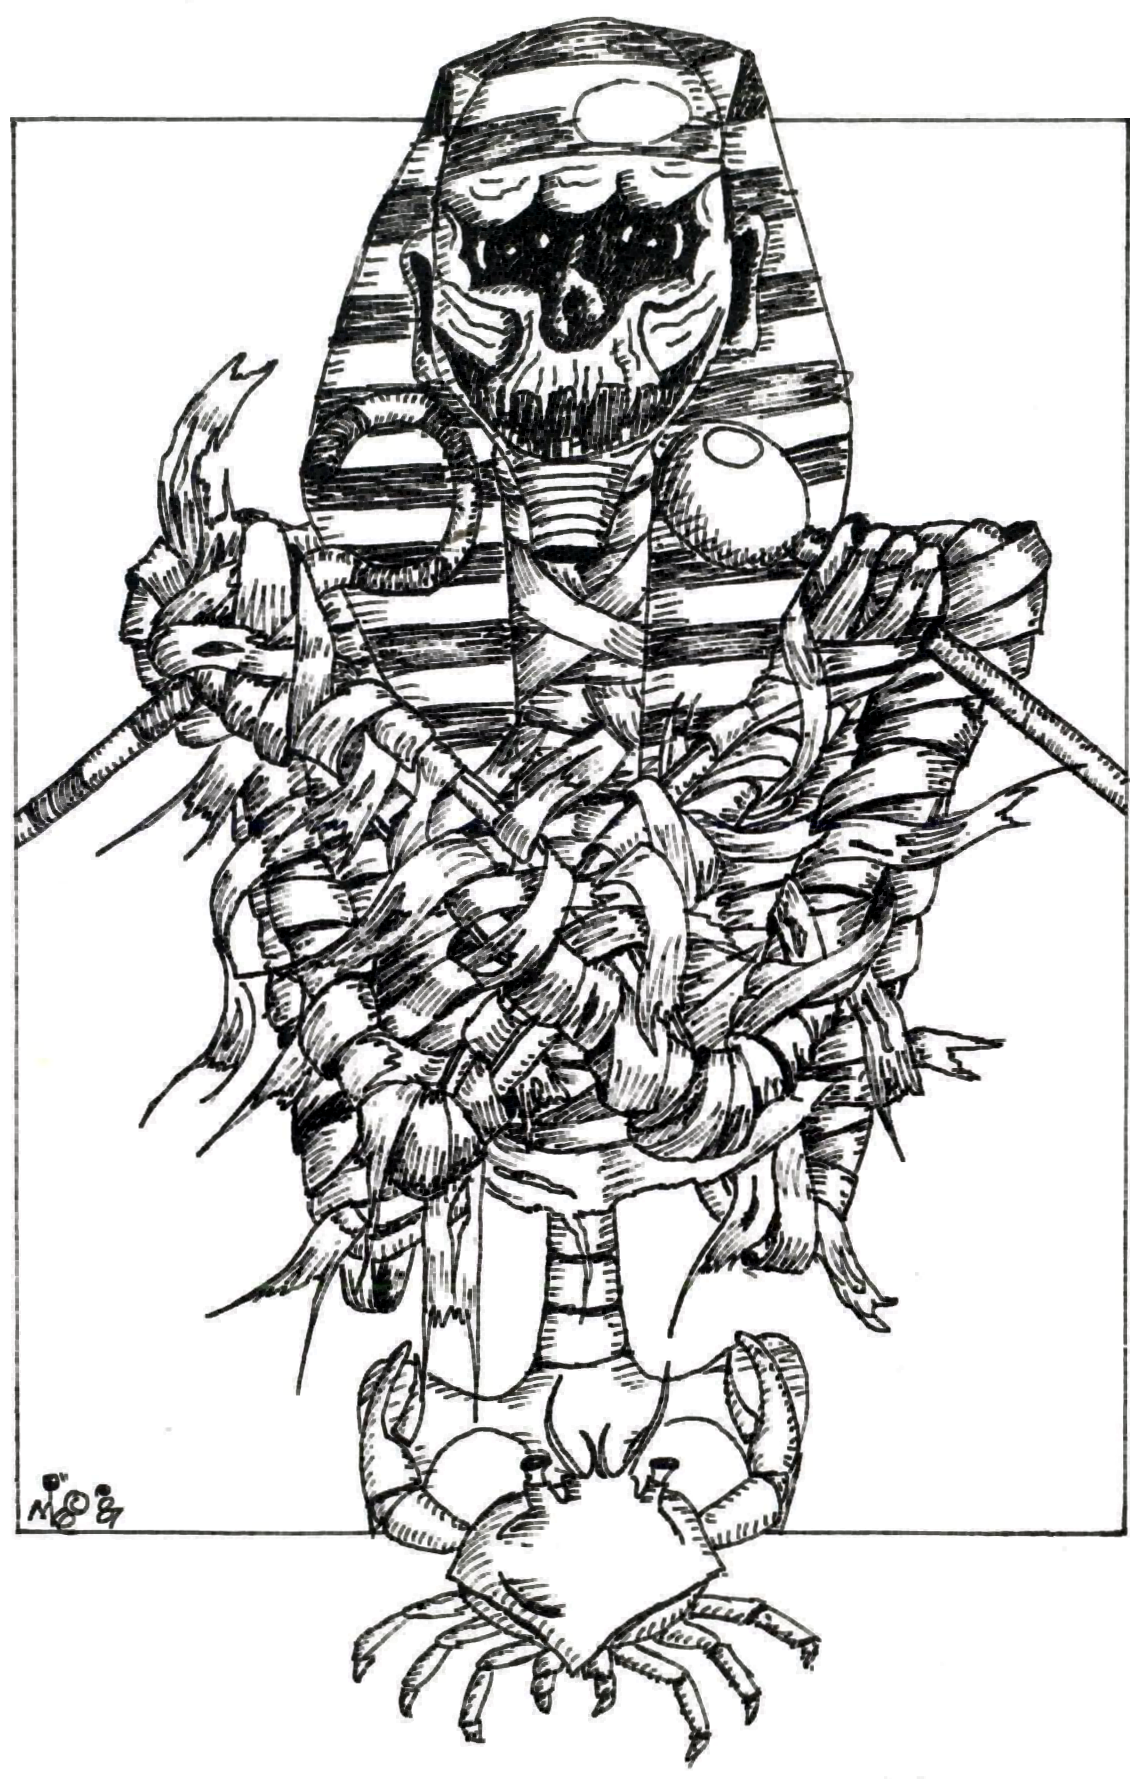
\includegraphics[width=\columnwidth]{rpg-module-interior-art.png}
\center{Tomb It May Concern.\\
Image Copyright \copyright 1987, 2016 Michael Davis. All rights reserved.}
\label{img:tomb}
\end{figure}

\lipsum[7-8]

\subsection{The Court of Set's Wives} % Key area 7

\lipsum[9]

\subsubsection{Statue of Nephthys} % Key area 7a
\label{west_court}

The statue of Nephthys, Set's first wife, is 20' tall. She is styled as a very beautiful woman dressed in the
style of Egyptian royalty\ldots

\subsubsection{Statue of Taweret} % Key area 7b

The statue of Taweret, another of Set's wives, appears as a hippo-headed humanoid. Her upper torso is bare\ldots

\vdots

\setcounter{subsection}{13} % Skip areas 8-13

\subsection{Inner Sanctuary} % Key area 14
\label{inner_sanctuary}

This area is guarded by the priest of Set, Snefru-hotep, and four Minions of Set!
\begin{statblockfreestyle}
\begin{ifbasicstats}
Snefru-hotep, Cleric of Set, S9 I15 W17 D10 C8 Ch15. AC 5 (chain mail), C5, hp 21, MV 90'\,(30'), Att mace, D 1--6, Save C5, ML 11, AL C.
He can cast the following spells: Protection from Good, Cause Fear, Snake Charm, Hold Person.
\end{ifbasicstats}
\begin{if1estats}
Snefru-hotep, Cleric of Set, S9 I15 W17 D10 C8 Ch15. AC 5 (chain mail), C5, hp 21, MV 9", Att mace, D 2--7, AL LE.
He can cast the following spells: Protection from Good, Cause Fear, Cause Light Wounds ($\times 2$), Darkness,
Snake Charm, Hold Person, Slow Poison, Spiritual Hammer, Speak with Animals, Animate Dead, Curse.
\end{if1estats}
\end{statblockfreestyle}
\statblock{minion_set}{4}{25 each}
\lipsum[10-11]

%%%%% Page break and switch to one-column mode %%%%%

\onecolumninline{\part{Second Dungeon Level}

The rpg-module class allows you to switch between double- and single- column modes within your document. The
\texttt{\textbackslash onecolumn} command will cause a page break and switch to one-column mode. Likewise,
the \texttt{\textbackslash twocolumn} command will cause a page break and switch back to two-column mode.

To mix one- and two-column text on the same page, you have two options. The \texttt{\textbackslash onecolumninline}
command takes one parameter, which is the text to typeset in single-column mode. This command causes a page
break, typesets the single-column text at the top of the page, then continues in two-column mode as before. This
text has been set using \texttt{\textbackslash onecolumninline}.

The second option is to use the \texttt{onecolumnfloat} environment, which creates a \LaTeX~float the full width
of a page. This can be positioned using the usual float parameters, e.g. \texttt{[t]} for the top of the page
and \texttt{[b]} for the bottom. This option is most suitable where you want to have a table or ``sidebar'' text
which is separate from your main text body. You can float graphics in the same way using the
\texttt{figure*} environment, as we do for the map on p.\pageref{img:map}.

It is not possible to mix \texttt{\textbackslash onecolumninline} and \texttt{\textbackslash onecolumnfloat} on
the same page.

\section*{Wandering Monsters}
\label{wanderingmonsters}

% Change the alignment of Acolytes from ``Any'' to ``Chaotic''

%\changealignment{acolyte}{Chaotic}
\changealignment{acolyte}{LE}

\begin{wanderingmonsters}[b]
\wanderitem{crocodile}{1--2}
\wanderitem{rock_baboon}{}
\wanderitem{pit_viper}{}
\wanderitem[4-6]{gnoll}{}
\wanderitem[7-8]{acolyte}{}
\wanderitem[9]{minion_set}{1}
\wanderitem{snefru_hotep}{}
\end{wanderingmonsters}

\section*{Monster Roster}

\begin{monsterroster}
\rosteritem{\ref{portico}}{gnoll}{6}{9 each}
\rosteritem{\ref{inner_sanctuary}}{snefru_hotep}{1}{21}
\rosteritem{\ref{inner_sanctuary}}{minion_set}{4}{25 each}
\end{monsterroster}
} % end of \onecolumninline

\noindent\lipsum[12-14]

\section{Concluding the Adventure}

\lipsum[12-13]

\newpage

%
% New Monsters part
%

\part{New Monsters}

% If you had a picture of a minion of set you could include it here
%\includegraphics[width=\linewidth]{minion_of_set.jpg}

\begin{newmonster}{minion_set}\label{minion_set}%
Minions of Set serve their master, the god of evil and the night, with unswerving devotion. In combat, they
never need to check morale. They are the implacable enemies of the servants of Osiris and Horus.

In human form, the Minions of Set wear scaly black plate armour and weild curved khopesh swords. Once per
day, they can polymorph themselves into the form of a giant snake with a poisonous bite. Some minions can
transform themselves into cave bears, giant crocodiles or giant scorpions.
\end{newmonster}

\part{License Information}

The \LaTeX~rpg-module class is Copyright \copyright 2016 Michael Davis and is distributed under the terms of the
\href{http://www.latex-project.org/lppl.txt}{LaTeX Project Public License} (LPPL) Version 1.3c.

You are free to use the class to generate works for your own private use and/or for distribution as detailed in
Clause 3 of the license. There is no restriction on commercial use.

An acknowledgement is much appreciated: you can use the \verb|\modulecopyright| macro to insert an acknowledgement
block. No payment is required or expected, but if you become extremely wealthy from the sales of a module
you typeset using this class and wish to express your appreciation you are welcome to do so via
\href{https://paypal.me/slithy}{PayPal}.

%
% License section
%

\section{Open Game Content}
\label{ogl}

The template includes three macros to make it easy to distribute your work under the Open Game License
from Wizards of the Coast: \verb|\ogl|, \verb|\productidentity| and \verb|\opengamecontent|. These three
macros produce the license text below:

\begin{ogl}
% This environment includes the complete text of the OGL v1.0A. Within the environment, you should include
% the exact text of the COPYRIGHT NOTICE of any other OGL text you are copying, modifying or distributing.
% Usually this will include the title, copyright date and copyright holder's name(s). Example:
\item System Reference Document, Copyright \copyright 2000--2003, Wizards of the Coast, Inc., by Jonathan Tweet, Monte Cook,
Skip Williams, Rich Baker, Andy Collins, David Noonan, Rich Redman, Bruce R. Cordell, John D. Rateliff, Thomas Reid, James
Wyatt, based on original material by E. Gary Gygax and Dave Arneson.
\end{ogl}

\begin{productidentity}
\item The text of this \LaTeX~rpg-module class and example template, which comprises all typesetting elements and all text which
is not explitly Open Game Content, is Product Identity.
\modulecopyright

\item All photographs, artwork and maps in this template are Product Identity.

\item The cover image is adapted from an original image on
\href{https://commons.wikimedia.org/wiki/File:Karnak_Tempel_Vorhof_05.jpg}{Wikimedia Commons}, copyright \copyright 2009 Olaf
Tausch. Used with permission under the terms of the
\href{https://creativecommons.org/licenses/by/3.0/deed.en}{Creative Commons Attribution 3.0 Unported} license.

\item The map on p.\pageref{img:map} is copyright \copyright 2008, 2016 Tim Hartin of \href{http://paratime.ca}{Paratime Design}.
Used with permission. All rights reserved.

\item The drawing on p.\pageref{img:tomb} is copyright \copyright 1987, 2016 Michael Davis. All rights reserved.
\end{productidentity}

\begin{opengamecontent}
\item The monster statistics from the SRD are Open Game Content.
\end{opengamecontent}

\newpage

%
% Table of Contents
%

\tableofcontents

% If you would also like to include an index for your document, see the LaTeX makeidx package

\end{document}
